
\documentclass[10pt]{article}

\usepackage{authblk}
\usepackage[T1]{fontenc}
\usepackage[utf8]{inputenc}
\usepackage{setspace}
\usepackage{graphics}
\usepackage{graphicx}
\usepackage{xspace,url,cite}
\usepackage{fancyvrb}
\usepackage{boxedminipage}
\usepackage{epsfig}
\usepackage{multirow}
\usepackage{bbm}
\usepackage{eufrak}
\usepackage{textcomp}
\usepackage{mathtools}
\usepackage{amssymb}
\usepackage{amsthm}
\usepackage{mathrsfs}
\usepackage[papersize={8.5in,11in},text={6.5in,9in}]{geometry}
\usepackage[cal=boondoxo]{mathalfa}
\usepackage{xfrac}
\usepackage{float}
\usepackage{listings}
\usepackage{xcolor}
\usepackage{fancyhdr}
\usepackage{subcaption}

\definecolor{codegreen}{rgb}{0,0.6,0}
\definecolor{codegray}{rgb}{0.5,0.5,0.5}
\definecolor{codepurple}{rgb}{0.58,0,0.82}
\definecolor{backcolour}{rgb}{0.95,0.95,0.92}

\lstdefinestyle{mystyle}{
    backgroundcolor=\color{backcolour},   
    commentstyle=\color{codegreen},
    keywordstyle=\color{magenta},
    numberstyle=\tiny\color{codegray},
    stringstyle=\color{codepurple},
    basicstyle=\ttfamily\footnotesize,
    breakatwhitespace=false,         
    breaklines=true,                 
    captionpos=b,                    
    keepspaces=true,                 
    numbers=left,                    
    numbersep=5pt,                  
    showspaces=false,                
    showstringspaces=false,
    showtabs=false,                  
    tabsize=2
}
\lstset{style=mystyle}

\pagestyle{fancy}
\fancyhead[L]{W233}
\fancyhead[C]{Project Proposal}
\fancyhead[R]{Group \#2}
\fancyfoot[L]{}
\fancyfoot[C]{}
\fancyfoot[R]{\thepage}
\fancypagestyle{firstpage}{%
  \fancyhf{}% clear default for head and foot
  \lhead{W233}
  \chead{Privacy Engineering}
  \rhead{Fall 2022}
}
\usepackage{xpatch}
\xapptocmd{\titlepage}{\thispagestyle{firstpage}}{}{}

% https://tex.stackexchange.com/questions/130762/prl-style-horizontal-line-in-latex
% \newcommand{\titleseparator}{\noindent\makebox[\linewidth]{\resizebox{0.75\linewidth}{1.5pt}{$\bullet$}}\bigskip}
% \newcommand{\sectionseparator}{\noindent\makebox[\linewidth]{\resizebox{0.5\linewidth}{1pt}{$\bullet$}}\bigskip}
% \newcommand{\problemseparator}{\noindent\makebox[\linewidth]{\resizebox{0.3\linewidth}{0.75pt}{$\bullet$}}\bigskip}
% \newcommand\numberthis{\addtocounter{equation}{1}\tag{\theequation}}

% \renewcommand{\thesection}{Problem \arabic{section}}
% \renewcommand{\thesubsection}{\arabic{section}(\alph{subsection})}

% https://tex.stackexchange.com/questions/466066/font-size-confusion-in-latex
\renewcommand{\Affilfont}{\footnotesize}
\renewcommand{\Authfont}{\normalsize}

% https://tex.stackexchange.com/questions/216098/redefine-maketitle
\makeatletter
\def\@maketitle{%
  \newpage
  \null
  %\vskip 2em%
  \begin{center}%
  \let \footnote \thanks
    {\LARGE \@title \par}%
    %\vskip 1.5em%
    \vskip 1em
    {\large
      \lineskip .5em%
      \begin{tabular}[t]{c}%
        \@author
      \end{tabular}\par}%
    \vskip 0.51em%
    %{\large \@date}
  \end{center}%
  \par
  %\vskip 1.5em
  \vskip 0.5em}
\makeatother

\begin{document}

\title{Authenticity and Confidentiality in Sharing Digital Objects\\
\large Identify Plagiarism in Digital Photography}
%\author{Amangeet Samra \and Amrita Mande \and Catherine Jimerson \and Diamond Rorie \and Mahesh Arumugam}

\author{Amangeet Samra}
\author{Amrita Mande}
\author{Catherine Jimerson}
\author{Diamond Rorie}
\author{Mahesh Arumugam}
\affil[]{W233 Project Group \#2}

\maketitle
\thispagestyle{firstpage}   

\section{Problem Statement}
\label{sec:stmt}

We propose investigating the authenticity and confidentiality aspects of sharing digital objects, especially digital photographs, in news publications. More specifically, in the context of recent fake news proliferation, we aim to address the problem of ensuring authenticity to a published photograph while remaining anonymous both to the news publisher and the reader. The project aims to design and implement a system that provides robust confidentiality to a source of a digital object while allowing a publisher to authenticate the object through a trusted authority for authenticity (i.e., original and not fabricated beyond acceptable edits) and verify that the source is the owner of the object. In addition, the project aims to construct a {\em lineage} of the edits and measure the difference between the objects. In this project, we consider the following use cases.

\begin{enumerate}
\item {\em The owner claims ownership of the object.} For example, a well-known photographer wants to copyright the photographs.
\item {\em The owner renounces their ownership of the object.} For example, a photographer clicks a photograph of some compromising scenario. And the owner does not prefer to be associated with the click. 
\end{enumerate}

\section{Literature Review}

Since we focus on the authenticity and confidentiality aspects of sharing objects, we investigated existing work on these two aspects. 

\begin{enumerate}
\item {\bf The case for the confidentiality of the source. } Historically, from the journalism perspective, sources should only be confidential when necessary \cite{wulfemeyer83}. Now the ability of the internet to ruin a person's life for a perceived slight or membership to a certain group is a given; everyday people wonder if they will become the next internet's most wanted \cite{svana18}. In the age of internet confidentiality, privacy has never been more prized and more easily subverted \cite{durity05,svana18}. Frameworks exist that provide sharing pathways where the pathways do not identify the users \cite{cvppfr19, tccn13}. Tangentially, we propose a system that provides confidentiality to the source (if desired) while allowing the reporter or any other third party to authenticate the originality and volume of edits done to the piece of media (the main use case being digital photographs).
\item {\bf The case for authenticity.} The proliferation of ``deep fakes'' in the media has created a need for any third party that wants to take a piece of media and use it to check the providence thoroughly \cite{ckdg20}. Providence and edit checking are available to experts in their related fields \cite{cooper10}, but may be unusable or impractical for journalists or, say, an art expert who wants to know that they are buying authentic digital art \cite{wlwc21}. In addition, other mechanisms (including Blockchain, e.g., \cite{qqjs19}) address fake news using a verification framework that involves all the actors (the source, the publisher, and the reader).  
\end{enumerate}

\section{Preliminary Architecture and Proposal}

Figure \ref{fig:arch} shows the preliminary architecture of our system. Next, we discuss the architecture for the two use cases we identified in Section \ref{sec:stmt}.

\begin{figure}[H]
\centering
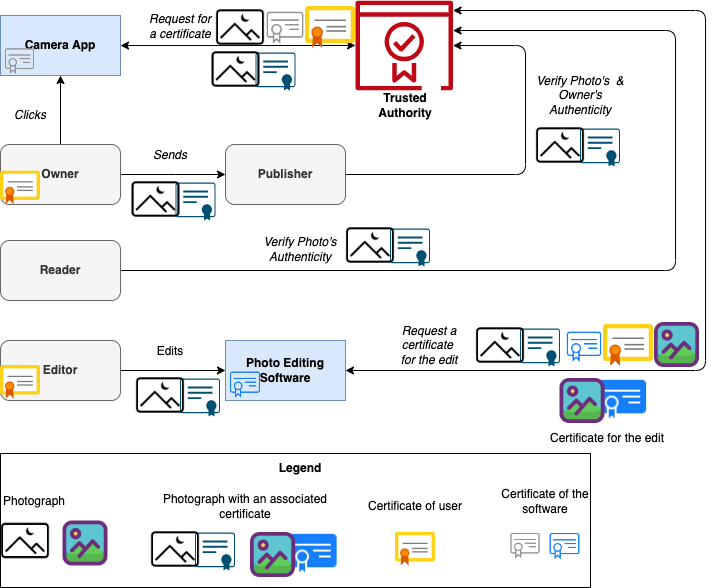
\includegraphics[scale=0.38]{arch.png}
\caption{Proposed architecture of the system}
\label{fig:arch}
\end{figure}

\noindent{\bf The owner claims ownership of the object.}
\begin{enumerate}
\item Owner takes a picture using a camera app and requests a certificate from a Trusted Authority ({\em TA}).
\item The TA successfully issues the certificate. 
\item Upon being sent to the publisher, the photo's authenticity is cross-verified with the TA.
\item A reader can also verify the photo's authenticity with the TA. 
\item On edit of a photograph, the TA will issue a new certificate depending on the level of edits. 
\end{enumerate}

\noindent{\bf The owner renounces their ownership of the object. }
\begin{enumerate}
\item Suppose the owner does not prefer to be associated with the click. The TA issues the certificate without associating that with the user certificate. For example, if a person sees a celebrity engage in dangerous behavior, there is value in holding the celebrity accountable. However, the person must account for their safety against the fanbase. 
\item Owner chooses to remain anonymous, in which case the publisher will accept the denounced owner role and verify the certificate with the TA. 
\item A reader can also verify the photo's authenticity with the TA. 
\item On edit of a photograph, the TA will issue a new certificate depending on the level of edits. 
\end{enumerate}

\section{Potential Contributions from Each Member}

Table \ref{tbl:contributions} identifies each group member's potential contributions. The team will review these commitments throughout the project and make appropriate adjustments. In addition, the team communications agreement document is available at \url{https://bit.ly/3SK5MEC}.

\begin{table}[H]
\small
\begin{center}
\begin{tabular}{|l||l|}
\hline
Member & Potential Contributions\\
\hline
\hline
Amangeet Samra                      & Coding and final paper discussion\\\hline
Amrita Mande                        & Architecture, uses case development, and coding\\\hline
Catherine Jimerson                  & Final paper (including methods, results, literature review) and coding\\\hline
Diamond Rorie                       & Literature review and final paper (including motivation survey of related work)\\\hline
Mahesh Arumugam                     & Architeture, typesetting of the final paper, Grammarly verification, and coding. \\\hline
\end{tabular}
\caption{Potential contributions from each member of Group \#2}
\label{tbl:contributions}    
\end{center}
\end{table}

\section{Proposed Milestones}

Table \ref{tbl:milestones} identifies the project milestones, deliverables, and deadlines. 

\begin{table}[H]
\small
\begin{center}
\begin{tabular}{|l|l||c|}
\hline
Milestone & Description & Expected ETA\\
\hline
\hline
Project proposal                    & Project proposal submission & September 30, 2022\\\hline
\multirow{3}{*}{Checkpoint \#1}     & 1. Finalize use cases & \multirow{3}{*}{October 19, 2022}\\
                                    & 2. Review and finalize architecture and workflow & \\
                                    & 3. Design APIs for components & \\\hline
\multirow{3}{*}{Mid-term review}    & 1. Preliminary project presentation \& report review  & \multirow{3}{*}{November 4, 2022}\\
                                    & 2. Progress and adjustments if needed & \\
                                    & 3. Coding components of the system & \\\hline
\multirow{2}{*}{Checkpoint \#2}     & 1. Coding complete and integration testing & \multirow{2}{*}{November 23, 2022}\\
                                    & 2. Draft project report & \\\hline
Presentation rehearsal              & Project presentation rehearsal & November 30, 2022\\\hline
Class project presentation          & Class presentation & Week of December 5, 2022 \\\hline
Final paper review                  & Final paper review & Week of December 5, 2022\\\hline
Final project paper                 & Final project report submission & December 9, 2022\\\hline
\end{tabular}
\caption{Proposed milestones of the project}
\label{tbl:milestones}    
\end{center}
\end{table}

\footnotesize
\bibliography{proposal}
\bibliographystyle{unsrt}


\end{document}
